\documentclass[a4paper,10pt]{article}
\usepackage[margin=1.4in]{geometry}
\usepackage[swedish]{babel}
\usepackage[utf8]{inputenc}
\usepackage{titlesec}
\usepackage{titling}
\usepackage{todonotes}



\setlength{\parskip}{1em}
\setlength{\parindent}{0pt}
\titlespacing{\section}{0pt}{\parskip}{-\parskip}
\titlespacing{\subsection}{0pt}{\parskip}{-\parskip}
\titlespacing{\subsubsection}{0pt}{\parskip}{-\parskip}
\titlespacing{\part}{0pt}{\parskip}{-\parskip}

\usepackage{graphicx}
\usepackage{adjustbox}

\begin{document}
\def\ftitle{Arkitekturdokument}
\def\fversion{1.0}
\begin{titlepage} % Suppresses displaying the page number on the title page and the subsequent page counts as page 1
	\newcommand{\HRule}{\rule{\linewidth}{0.5mm}} % Defines a new command for horizontal lines, change thickness here

	\center % Centre everything on the page

	%------------------------------------------------
	%	Headings
	%------------------------------------------------

	\textsc{\LARGE Linköpings universitet \\ \vspace{0.2em} Institutionen för datavetenskap }\\[2cm]

    \large\today

    \vspace{1cm}


	%------------------------------------------------
	%	Title
	%------------------------------------------------

	\HRule\\[0.4cm]

	{\huge\bfseries Schemaläggningsstöd för  kirurgi \vspace{.1em} \\ \ftitle }\\[0.4cm] % Title of your document

	\HRule\\[1cm]

	%------------------------------------------------
	%	Author(s)
	%------------------------------------------------

	\begin{minipage}{0.7\textwidth}
			\large
            \emph{Version: \fversion}
            \vspace{1em}

            \textbf{\\Adam Andersson, Niclas Byrsten, \\Björn Hvass, Henrik Lindström, \\Martin Persson, Christoffer Sjöbergsson, \\Tor Utterborn}


            \vspace{1em}

            Handledare: Jonas Wallgren

            Examinator: Kristian Sandahl
	\end{minipage}
	~

	%------------------------------------------------
	%	Logo
	%------------------------------------------------

	%\vfill\vfill
	%
\includegraphics[width=0.2\textwidth]{../Templates/Aeon}\\[1cm] % Include a department/university logo - this will require the graphicx package

	%----------------------------------------------------------------------------------------

	\vfill % Push the date up 1/4 of the remaining page

\end{titlepage}


\section*{\begin{center}Projektidentitet\end{center}}
    \vspace{-2.5em}
    \begin{center}
        \begin{tabular}{|c c c|}
        \hline
        Namn & Roll & E-post \\
        \hline
        Adam Andersson& Teamleader & adam.e.a.andersson@gmail.com\\
        \hline
        Niclas Byrsten & Testansvarig & nicby889@student.liu.se\\
        \hline
        Björn Hvass & Konfigurationsansvarig & bjorn.hvass@gmail.com\\
        \hline
        Henrik Lindström & Utvecklingsledare & henli070@student.liu.se\\
        \hline
        Martin Persson & Arkitekturansvarig & marpe902@liu.student.se\\
        \hline
        Christoffer Sjöbersson & Analysansvarig & chrsj812@liu.student.se\\
        \hline
        Tor Utterborn & Dokument- \& Kvalitetsansvarig & tor.utterborn@gmail.com\\
        \hline
        \end{tabular}
    \end{center}

    \begin{center}
        \small
        \textbf{Kund}\\Region Östergötland, 581 91 Linköping.

        \textbf{Kontaktperson hos kund}\\
        Gunnar Nordqvist, IT-arkitekt, 010-1030698, Gunnar.Nordqvist@regionostergotland.se\\
        Erik Sundvall, Informationsarkitekt, 010-1036252, Erik.Sundvall@regionostergotland.se
    \end{center}

\vspace{9em}



\section*{\begin{center}Dokumentationshistorik\end{center}}
\begin{center}
 \begin{tabular}{|c c c c |}
 \hline
 Datum & händelse & iteration & version\\
 \hline
 2018-02-10 & Dokument skapas & 1 &  0.1\\
 \hline
  2018-02-19 & Konvertering till \textbf{\LaTeX} & 1 &  0.2\\
 \hline
   2018-02-19 & Version 1.0 färdigställd & 1 &  1.0\\
 \hline
\end{tabular}
\clearpage
\end{center}
\tableofcontents
\clearpage
\section{Inledning}
\label{sec:Inledning}

\subsection{Syfte}
Arkitekturdokumentet ger en utförlig översikt  av schemaläggningssystemets arkitektur. I dokumentet presenteras flera olika vyer av arkitekturen samt en översiktlig beskrivning av systemet och dess funktionalitet.
\subsection{Översiktlig systembeskrivning}
Det schemaläggningssystem som ska utvecklas kommer användas på operationsavdelningen i ett sjukhus av sjukhuspersonal för planering av operationer. Systemet ska klara av att utifrån en lista med beslutade operationer ge användaren förslag på operationstider inom operationens tidsgräns då rätt lokal och resurser finns tillgängliga. För tider då lokal finns att tillgå men resurser saknas ska systemet visa vilka resurser som saknas. Användaren ska utifrån detta kunna välja en passande tid och boka in operationen. Besluten ska innehålla relevant data om patient och operationstyp, och det ska för varje beslut framgå om beslutet behandlats eller inte. Ifall patienten behöver flera ingrepp ska användaren kunna se detta och kunna slå samman ingreppen till en operation vid behov.

Operationer ska kunna avbokas och frigöras från schemat. Det ska finnas en schemaöversikt med en filterfunktion som visar när vilka resurser är lediga eller upptagna. Det ska finnas en tidslinje över operationen som visar när operationsprocessens olika stadier börjar. Det ska gå att logga vilken användare som bokat vad. All information ska lagras i en central databas. Från databasen ska informationen hämtas ned till användardatorer via en server. Systemet ska visas på en skärm och användaren interagerar med det med hjälp av tangentbord och mus.

\section{Användarfallsvy}

Denna vy visar de viktigaste fallen då schemaläggningssystemet ska användas. De fallen är som följer:
\begin{itemize}
	\item Inloggning
	\item Visa tidslinje för operation
	\item Visa beslutsöversikt
	\item Visa beslutsdata
	\item Boka operation
	\item Avboka operation
	\item Visa schemaöversikt
	\item Slå ihop operationer
\end{itemize}
\subsection{Användarfallsdiagram}
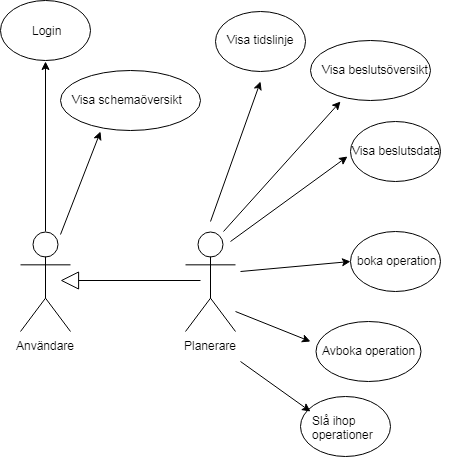
\includegraphics[width=\textwidth,height=\textheight,keepaspectratio]{Usecasediagram.png}
\clearpage
\section{Systemskiss}
\label{sec:Systemskiss}
Här visas och beskrivs en översiktlig skiss av schemaläggningssystemet där det framgår vilken funktionalitet som ska köras var i systemet. \\
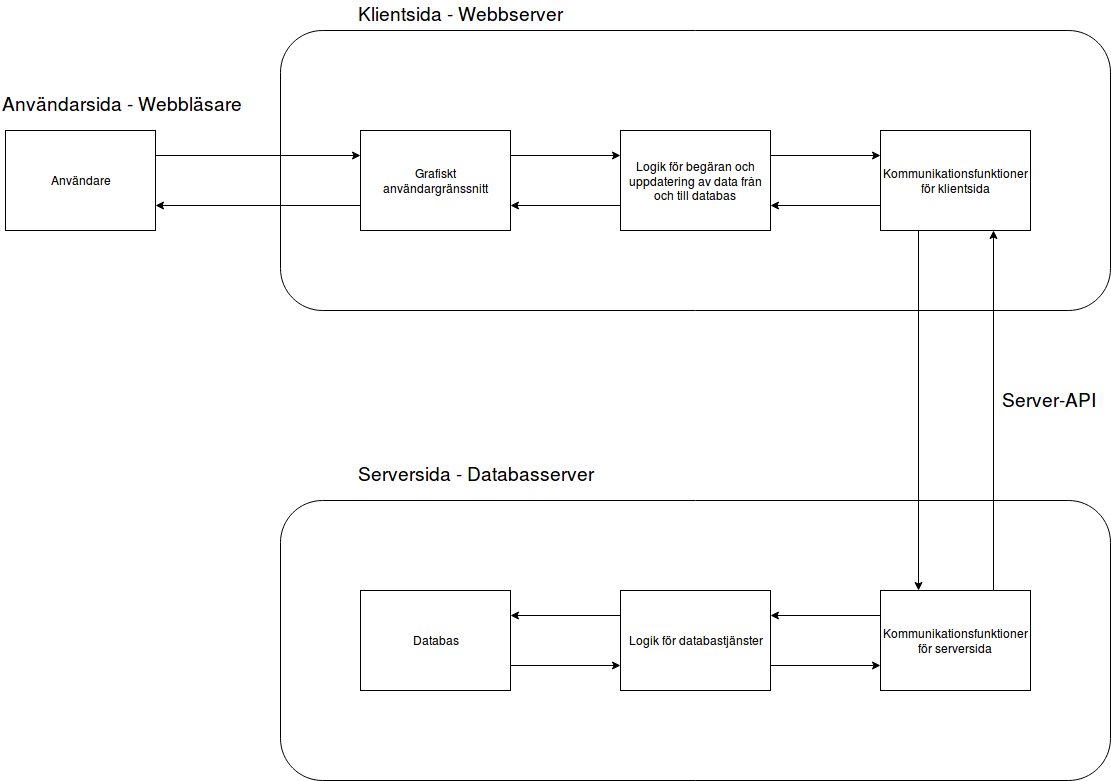
\includegraphics[width=.9\linewidth,height=.7\textheight]{Systemskiss.png}
\\
Systemet som beskrivs översiktligt i Figur 2 är uppdelat i två delar, en webbklient och en webbserver.
\section{Webbklient}
Webbklienten kommer att byggas på webbapplikationsramverket Angular. Den kommer att består av tre lager, ett gränssnittslager, ett logiklager och ett kommunikationslager. I klientdelen i Figur 2 beskrivs hur lagren hänger ihop och beror på varandra.

\subsection{Angular}
Denna sektion behandlar de delar ur Angulars arkitekturguide (referens till https://angular.io/guide/architecture) som kommer att vara relevanta i projektet.

En Angular-applikation är uppbyggd av en eller flera moduler som i sin tur består av komponenter och tjänster.
\subsubsection{Komponenter}
\label{komponent}
Angularkomponenter används för att dela upp gränssnittet i olika återanvändbara delar. Varje komponent ansvarar för en egen del av gränssnittet och består av dels en HTML-mall som beskriver dess utseende och dels en TypeScript-klass som hanterar allt det dynamiska med komponenten.

Komponentens mall definieras med hjälp av en något utökad HTML-syntax. All vanlig HTML förutom dess script-taggar får användas. Det tillkommer även en Angular-specifik syntax som tillåter mallen att anpassa sitt uteseende beroende på klassens tillstånd.
\subsubsection{Tjänster}
Tjänster i Angular är klasser, skrivna i TypeScript, som tillhandahåller funktioner och logik som krävs av modulens komponenter eller andra tjänster. Typiskt ska de ha ett smalt och väldefinierat syfte.

\subsection{Gränssnittslager}
Gränssnittslagret har hand om allt som har med användarupplevelse och grafik i applikationen. Det kommer uteslutande att bestå av Angluarkomponenter som beskrivna i sektion \ref{komponent}.

Varje komponent ska ha ett väldefinierat syfte och såvida den inte är trivial bör den vara uppdelad i andra mindre komponenter. Komponenternas klasser ska endast innehålla den logik som krävs för visning och interaktion med användaren. Alla andra funktioner som krävs men som inte direkt har med användarupplevelsen att göra ska finnas i komponenten, utan i tjänster som ligger i logiklagret.

\subsection{Logiklager}
   


%%Systemet som beskrivs översiktligt i Diagram 2 innehåller en webbserver som innehåller ett grafisk användargränssnitt. Logik på webbservern hanterar användarkommandon och uppdaterar grafiska komponenter. Slutligen innehåller webbservern kommunikationsfunktionalitet som gör det möjligt att skicka data till och ta emot data från databasservern. Användaren kör systemet via en webbläsare, Internet Explorer 11.

%%Systemet innehåller även en databasserver som kan ta emot data från och skicka data till webbservern och behandla den data som ligger i själva databasen. Användaren kör systemet från en webbläsare.


\end{document}
